%%=============================================================================
%% LaTeX sjabloon voor bachelorproef, HoGent Bedrijf en Organisatie
%% Opleiding Toegepaste Informatica
%%=============================================================================

\documentclass[fleqn,a4paper,12pt]{book}

%%=============================================================================
%% LaTeX sjabloon voor de bachelorproef, HoGent Bedrijf en Organisatie
%% Opleiding toegepaste informatica
%%
%% Structuur en algemene vormgeving. Meestal hoef je hier niets te wijzigen.
%%
%% Vormgeving gebaseerd op "The Legrand Orange Book", version 2.0 (9/2/15)
%% door Mathias Legrand (legrand.mathias@gmail.com) met aanpassingen door
%% Vel (vel@latextemplates.com). Het oorspronkelijke template is te vinden op
%% http://www.LaTeXTemplates.com
%%
%% Aanpassingen voor HoGent toegepaste informatica: 
%%   Bert Van Vreckem <bert.vanvreckem@hogent.be>
%% Licentie: 
%%   CC BY-NC-SA 3.0 (http://creativecommons.org/licenses/by-nc-sa/3.0/)
%%=============================================================================

%%-----------------------------------------------------------------------------
%% Packages
%%-----------------------------------------------------------------------------

\usepackage[top=3cm,bottom=3cm,left=3cm,right=3cm,headsep=10pt,a4paper]{geometry} % Page margins
\usepackage[utf8]{inputenc}  % Accenten gebruiken in tekst (vb. é ipv \'e)
\usepackage{amsfonts}        % AMS math packages: extra wiskundige
\usepackage{amsmath}         %   symbolen (o.a. getallen-
\usepackage{amssymb}         %   verzamelingen N, R, Z, Q, etc.)
\usepackage[english,dutch]{babel}    % Taalinstellingen: woordsplitsingen,
                             %  commando's voor speciale karakters
                             %  ("dutch" voor NL)
\usepackage{iflang}
\usepackage{eurosym}         % Euro-symbool €
\usepackage{geometry}
\usepackage{graphicx}        % Invoegen van tekeningen
\graphicspath{{img/}}       % Specifies the directory where pictures are stored
\usepackage{tikz}            % Required for drawing custom shapes
\usepackage[pdftex,bookmarks=true]{hyperref}
                             % PDF krijgt klikbare links & verwijzingen,
                             %  inhoudstafel
\usepackage{enumitem}        % Customize lists
\setlist{nolistsep}         % Reduce spacing between list items
\usepackage{listings}        % Broncode mooi opmaken
\usepackage{color}
\definecolor{lightgray}{rgb}{.9,.9,.9}
\definecolor{darkgray}{rgb}{.4,.4,.4}
\definecolor{purple}{rgb}{0.65, 0.12, 0.82}

\lstdefinelanguage{JavaScript}{
  keywords={typeof, new, true, false, catch, function, return, null, catch, switch, var, if, in, while, do, else, case, break},
  keywordstyle=\color{blue}\bfseries,
  ndkeywords={class, export, boolean, throw, implements, import, this},
  ndkeywordstyle=\color{darkgray}\bfseries,
  identifierstyle=\color{black},
  sensitive=false,
  comment=[l]{//},
  morecomment=[s]{/*}{*/},
  commentstyle=\color{purple}\ttfamily,
  stringstyle=\color{red}\ttfamily,
  morestring=[b]',
  morestring=[b]"
}

\lstset{
   language=JavaScript,
   backgroundcolor=\color{lightgray},
   extendedchars=true,
   basicstyle=\footnotesize\ttfamily,
   showstringspaces=false,
   showspaces=false,
   numbers=left,
   numberstyle=\footnotesize,
   numbersep=9pt,
   tabsize=2,
   breaklines=true,
   showtabs=false,
   captionpos=b
}


\usepackage{multirow}        % Tekst over verschillende cellen in tabellen
\usepackage{rotating}        % Tabellen en figuren roteren

\usepackage{booktabs}        % Required for nicer horizontal rules in tables

\usepackage{xcolor}          % Required for specifying colors by name
\definecolor{maincolor}{RGB}{0,147,208} % Define the main color used for 
                             % highlighting throughout the book
                             % 0, 147, 208 = officiële kleur HoGent FBO

% Paragraph style: no indent, add space between paragraphs
\setlength{\parindent}{0em}
\setlength{\parskip}{1em}

\usepackage{etoolbox}
\usepackage{titling} % Macros for title, author, etc
\usepackage{lipsum}          % Voor vultekst (lorem ipsum)

%----------------------------------------------------------------------------------------
%	FONTS
%----------------------------------------------------------------------------------------

\usepackage{avant} % Use the Avantgarde font for headings
%\usepackage{times} % Use the Times font for headings
\usepackage{mathptmx} % Use the Adobe Times Roman as the default text font together with math symbols from the Sym­bol, Chancery and Com­puter Modern fonts

\usepackage{microtype} % Slightly tweak font spacing for aesthetics
\usepackage[utf8]{inputenc} % Required for including letters with accents
\usepackage[T1]{fontenc} % Use 8-bit encoding that has 256 glyphs

%------------------------------------------------------------------------------
%	TITLE PAGE
%------------------------------------------------------------------------------

\newcommand{\inserttitlepage}{%
\begin{titlepage}
  \newgeometry{top=2cm,bottom=1.5cm,left=1.5cm,right=1.5cm}
  \begin{center}

    \begingroup
    \rmfamily
    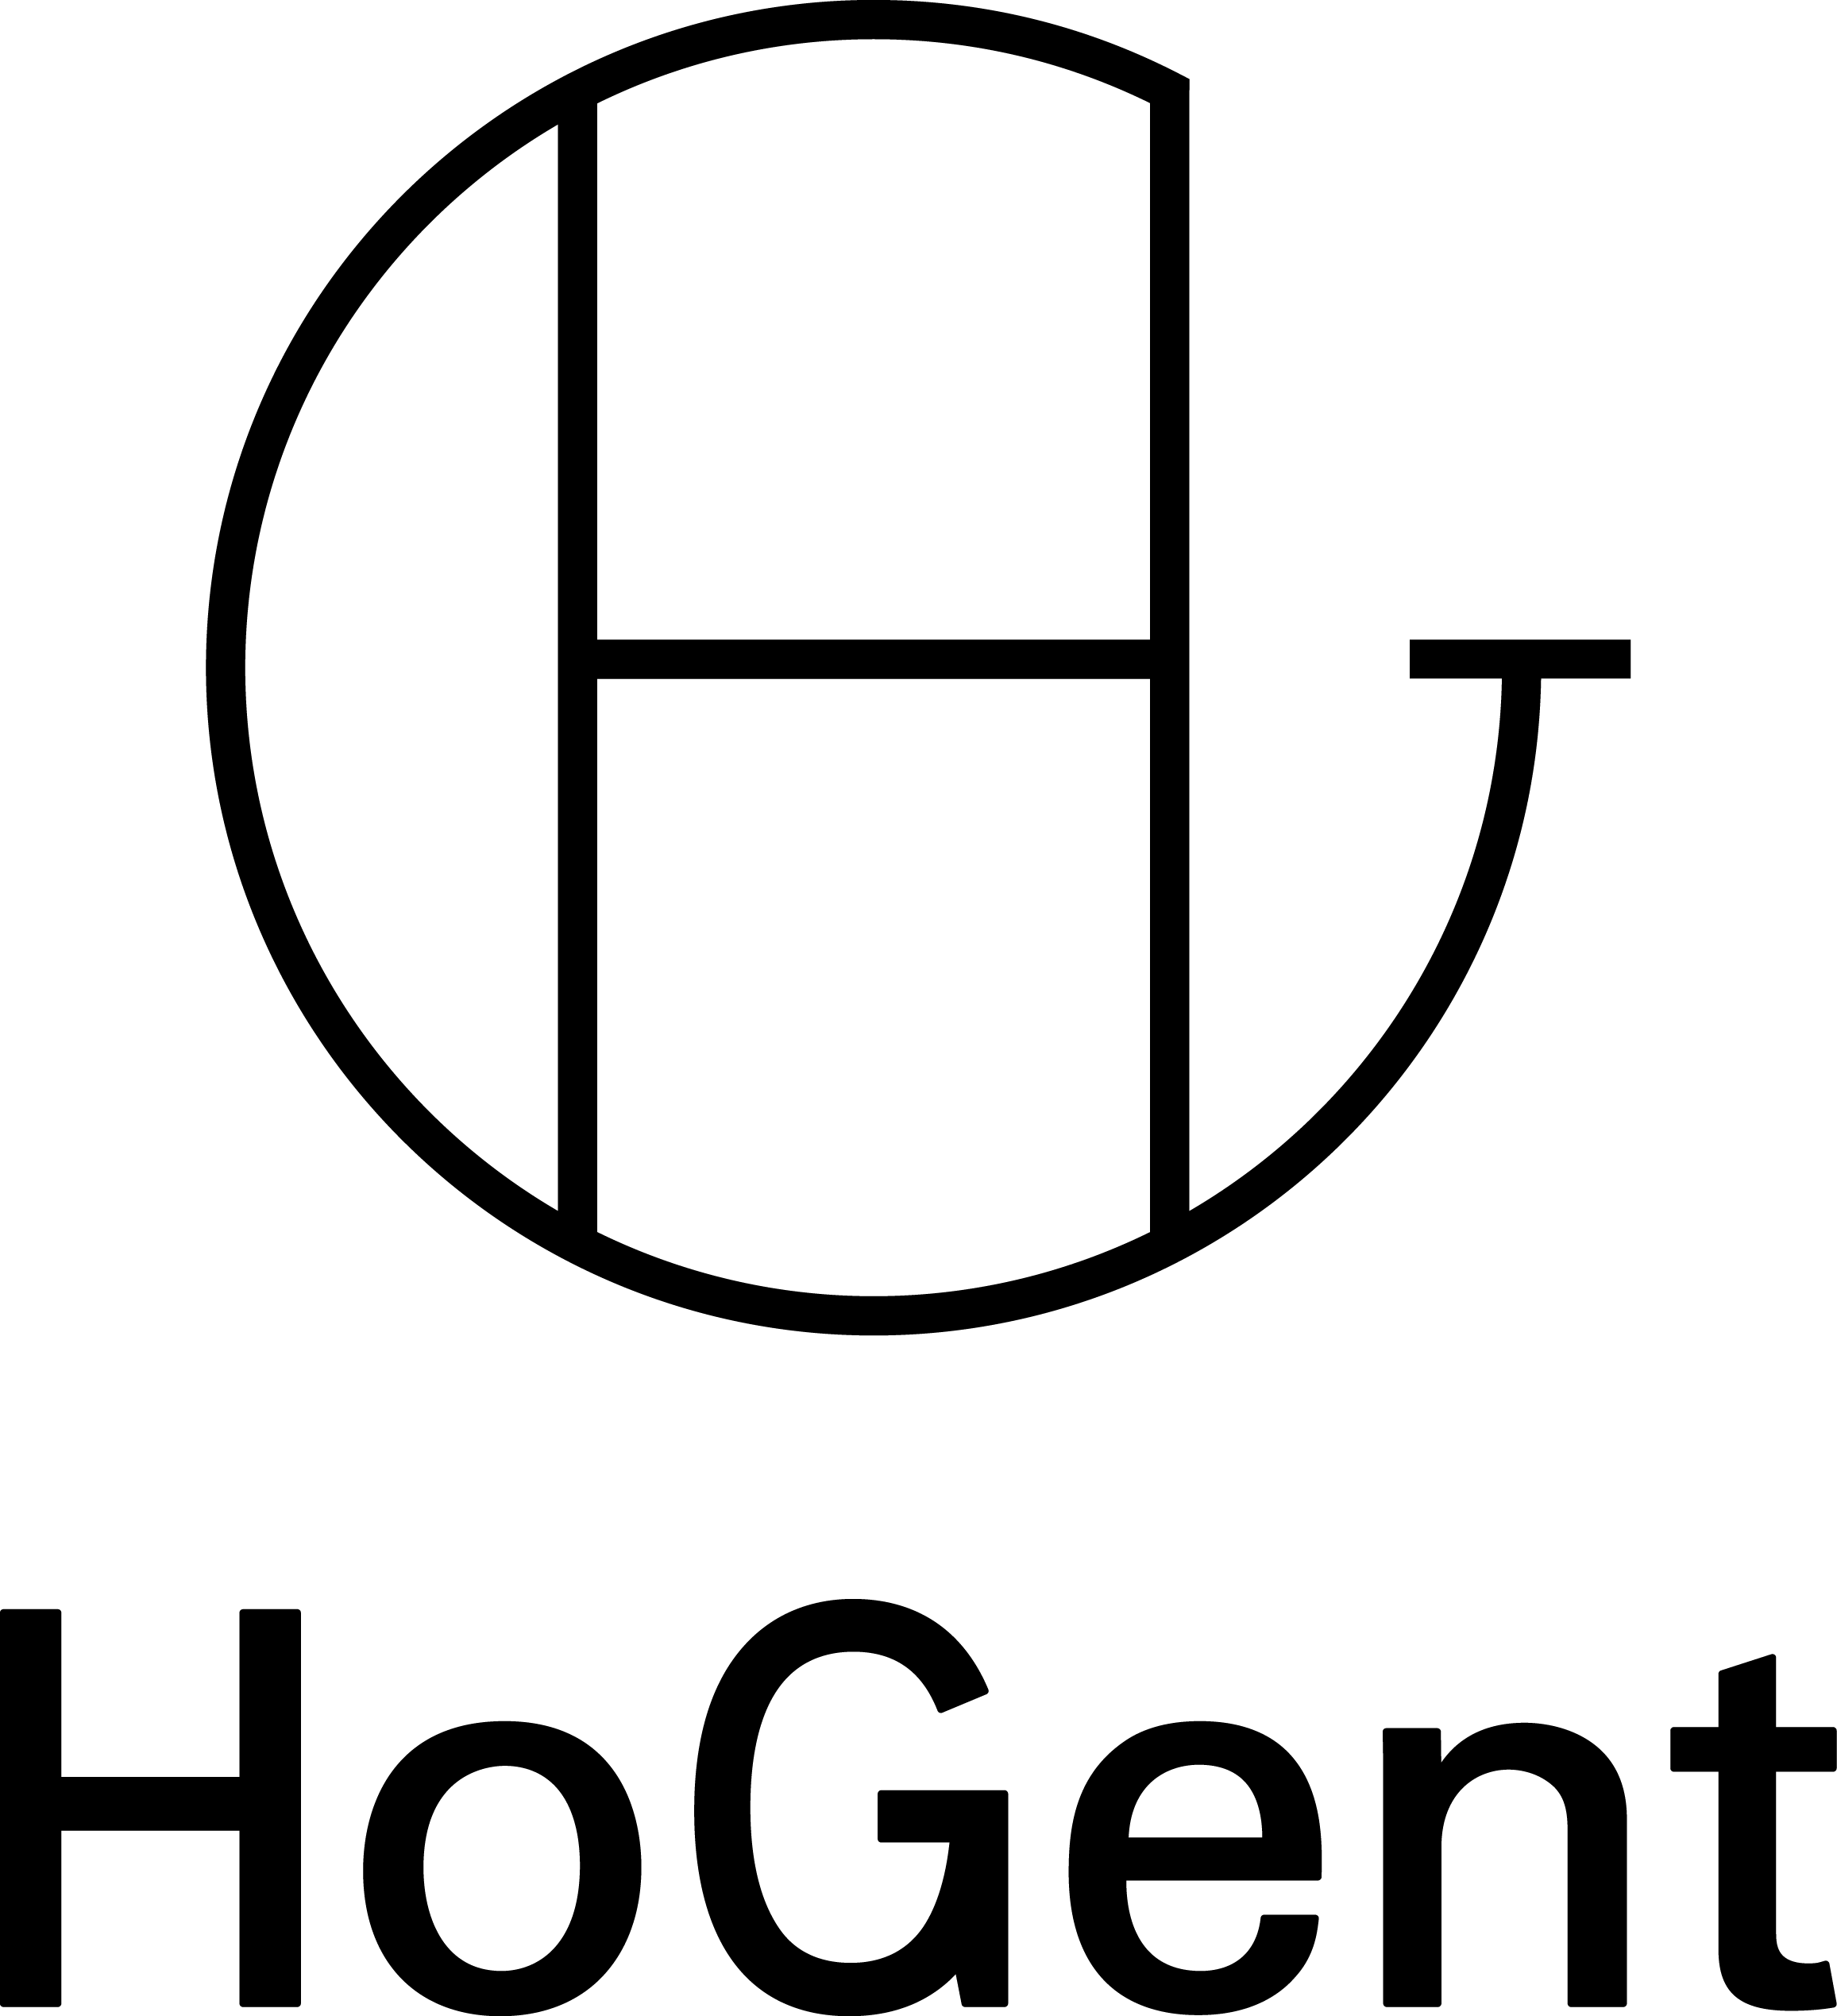
\includegraphics[width=2.5cm]{img/HG-beeldmerk-woordmerk}\\[.5cm]
    Faculteit Bedrijf en Organisatie\\[3cm]
    \titel
    \vfill
    \student\\[3.5cm]
    Scriptie voorgedragen tot het bekomen van de graad van\\professionele bachelor in de toegepaste informatica\\[2cm]
    Promotor:\\
    \promotor\\
    \ifdefempty{\copromotor}{\vspace{2.5cm}}{Co-promotor:\\\copromotor\\[2.5cm]}
    Instelling: \instelling\\[.5cm]
    Academiejaar: \academiejaar\\[.5cm]
    \ifcase \examenperiode \or Eerste \or Tweede \else Derde \fi examenperiode
    \endgroup

  \end{center}
  \restoregeometry
\end{titlepage}
  \emptypage
\begin{titlepage}
  \newgeometry{top=5.35cm,bottom=1.5cm,left=1.5cm,right=1.5cm}
  \begin{center}

    \begingroup
    \rmfamily
    \IfLanguageName{dutch}{Faculteit Bedrijf en Organisatie}{Faculty of Business and Information Management}\\[3cm]
    \titel
    \vfill
    \student\\[3.5cm]
    \IfLanguageName{dutch}{Scriptie voorgedragen tot het bekomen van de graad van\\professionele bachelor in de toegepaste informatica}{Thesis submitted in partial fulfilment of the requirements for the degree of\\professional bachelor of applied computer science}\\[2cm]
    Promotor:\\
    \promotor\\
    \ifdefempty{\copromotor}{\vspace{2.5cm}}{Co-promotor:\\\copromotor\\[2.5cm]}
    \IfLanguageName{dutch}{Instelling}{Institution}: \instelling\\[.5cm]
    \IfLanguageName{dutch}{Academiejaar}{Academic year}: \academiejaar\\[.5cm]
    \IfLanguageName{dutch}{%
    \ifcase \examenperiode \or Eerste \or Tweede \else Derde \fi examenperiode}{%
    \ifcase \examenperiode \or First \or Second \else Third \fi examination period}
    \endgroup

  \end{center}
  \restoregeometry
\end{titlepage}
}

%----------------------------------------------------------------------------------------
%	BIBLIOGRAPHY AND INDEX
%----------------------------------------------------------------------------------------

\usepackage[style=apa,backend=biber]{biblatex}
\usepackage{csquotes}
\DeclareLanguageMapping{dutch}{dutch-apa}
\addbibresource{bachproef-tin.bib} % BibTeX bibliography file
\addbibresource{../voorstel/voorstel.bib}
\defbibheading{bibempty}{}

\usepackage{calc} % For simpler calculation - used for spacing the index letter headings correctly
\usepackage{makeidx} % Required to make an index
\makeindex % Tells LaTeX to create the files required for indexing

%----------------------------------------------------------------------------------------
%	MAIN TABLE OF CONTENTS
%----------------------------------------------------------------------------------------

\usepackage{titletoc} % Required for manipulating the table of contents

\contentsmargin{0cm} % Removes the default margin

% Part text styling
\titlecontents{part}[0cm]
{\addvspace{20pt}\centering\large\bfseries}
{}
{}
{}

% Chapter text styling
\titlecontents{chapter}[1.25cm] % Indentation
{\addvspace{12pt}\large\sffamily\bfseries} % Spacing and font options for chapters
{\color{maincolor!60}\contentslabel[\Large\thecontentslabel]{1.25cm}\color{maincolor}} % Chapter number
{\color{maincolor}}
{\color{maincolor!60}\normalsize\;\titlerule*[.5pc]{.}\;\thecontentspage} % Page number

% Section text styling
\titlecontents{section}[1.25cm] % Indentation
{\addvspace{3pt}\sffamily\bfseries} % Spacing and font options for sections
{\contentslabel[\thecontentslabel]{1.25cm}} % Section number
{}
{\hfill\color{black}\thecontentspage} % Page number
[]

% Subsection text styling
\titlecontents{subsection}[1.25cm] % Indentation
{\addvspace{1pt}\sffamily\small} % Spacing and font options for subsections
{\contentslabel[\thecontentslabel]{1.25cm}} % Subsection number
{}
{\ \titlerule*[.5pc]{.}\;\thecontentspage} % Page number
[]

% List of figures
\titlecontents{figure}[0em]
{\addvspace{-5pt}\sffamily}
{\thecontentslabel\hspace*{1em}}
{}
{\ \titlerule*[.5pc]{.}\;\thecontentspage}
[]

% List of tables
\titlecontents{table}[0em]
{\addvspace{-5pt}\sffamily}
{\thecontentslabel\hspace*{1em}}
{}
{\ \titlerule*[.5pc]{.}\;\thecontentspage}
[]

%----------------------------------------------------------------------------------------
%	MINI TABLE OF CONTENTS IN PART HEADS
%----------------------------------------------------------------------------------------

% Chapter text styling
\titlecontents{lchapter}[0em] % Indenting
{\addvspace{15pt}\large\sffamily\bfseries} % Spacing and font options for chapters
{\color{maincolor}\contentslabel[\Large\thecontentslabel]{1.25cm}\color{maincolor}} % Chapter number
{}
{\color{maincolor}\normalsize\sffamily\bfseries\;\titlerule*[.5pc]{.}\;\thecontentspage} % Page number

% Section text styling
\titlecontents{lsection}[0em] % Indenting
{\sffamily\small} % Spacing and font options for sections
{\contentslabel[\thecontentslabel]{1.25cm}} % Section number
{}
{}

% Subsection text styling
\titlecontents{lsubsection}[.5em] % Indentation
{\normalfont\footnotesize\sffamily} % Font settings
{}
{}
{}

%----------------------------------------------------------------------------------------
%	PAGE HEADERS
%----------------------------------------------------------------------------------------

\usepackage{fancyhdr} % Required for header and footer configuration

\pagestyle{fancy}
\renewcommand{\chaptermark}[1]{\markboth{\sffamily\normalsize\bfseries\chaptername\ \thechapter.\ #1}{}} % Chapter text font settings
\renewcommand{\sectionmark}[1]{\markright{\sffamily\normalsize\thesection\hspace{5pt}#1}{}} % Section text font settings
\fancyhf{} \fancyhead[LE,RO]{\sffamily\normalsize\thepage} % Font setting for the page number in the header
\fancyhead[LO]{\rightmark} % Print the nearest section name on the left side of odd pages
\fancyhead[RE]{\leftmark} % Print the current chapter name on the right side of even pages
\renewcommand{\headrulewidth}{0.5pt} % Width of the rule under the header
\addtolength{\headheight}{2.5pt} % Increase the spacing around the header slightly
\renewcommand{\footrulewidth}{0pt} % Removes the rule in the footer
\fancypagestyle{plain}{\fancyhead{}\renewcommand{\headrulewidth}{0pt}} % Style for when a plain pagestyle is specified

% Removes the header from odd empty pages at the end of chapters
\makeatletter
\renewcommand{\cleardoublepage}{
\clearpage\ifodd\c@page\else
\hbox{}
\vspace*{\fill}
\thispagestyle{empty}
\newpage
\fi}

%----------------------------------------------------------------------------------------
%	THEOREM STYLES
%----------------------------------------------------------------------------------------

\usepackage{amsmath,amsfonts,amssymb,amsthm} % For math equations, theorems, symbols, etc

\newcommand{\intoo}[2]{\mathopen{]}#1\,;#2\mathclose{[}}
\newcommand{\ud}{\mathop{\mathrm{{}d}}\mathopen{}}
\newcommand{\intff}[2]{\mathopen{[}#1\,;#2\mathclose{]}}
\newtheorem{notation}{Notation}[chapter]

% Boxed/framed environments
\newtheoremstyle{maincolornumbox}% % Theorem style name
{0pt}% Space above
{0pt}% Space below
{\normalfont}% % Body font
{}% Indent amount
{\small\bf\sffamily\color{maincolor}}% % Theorem head font
{\;}% Punctuation after theorem head
{0.25em}% Space after theorem head
{\small\sffamily\color{maincolor}\thmname{#1}\nobreakspace\thmnumber{\@ifnotempty{#1}{}\@upn{#2}}% Theorem text (e.g. Theorem 2.1)
\thmnote{\nobreakspace\the\thm@notefont\sffamily\bfseries\color{black}---\nobreakspace#3.}} % Optional theorem note
\renewcommand{\qedsymbol}{$\blacksquare$}% Optional qed square

\newtheoremstyle{blacknumex}% Theorem style name
{5pt}% Space above
{5pt}% Space below
{\normalfont}% Body font
{} % Indent amount
{\small\bf\sffamily}% Theorem head font
{\;}% Punctuation after theorem head
{0.25em}% Space after theorem head
{\small\sffamily{\tiny\ensuremath{\blacksquare}}\nobreakspace\thmname{#1}\nobreakspace\thmnumber{\@ifnotempty{#1}{}\@upn{#2}}% Theorem text (e.g. Theorem 2.1)
\thmnote{\nobreakspace\the\thm@notefont\sffamily\bfseries---\nobreakspace#3.}}% Optional theorem note

\newtheoremstyle{blacknumbox} % Theorem style name
{0pt}% Space above
{0pt}% Space below
{\normalfont}% Body font
{}% Indent amount
{\small\bf\sffamily}% Theorem head font
{\;}% Punctuation after theorem head
{0.25em}% Space after theorem head
{\small\sffamily\thmname{#1}\nobreakspace\thmnumber{\@ifnotempty{#1}{}\@upn{#2}}% Theorem text (e.g. Theorem 2.1)
\thmnote{\nobreakspace\the\thm@notefont\sffamily\bfseries---\nobreakspace#3.}}% Optional theorem note

% Non-boxed/non-framed environments
\newtheoremstyle{maincolornum}% % Theorem style name
{5pt}% Space above
{5pt}% Space below
{\normalfont}% % Body font
{}% Indent amount
{\small\bf\sffamily\color{maincolor}}% % Theorem head font
{\;}% Punctuation after theorem head
{0.25em}% Space after theorem head
{\small\sffamily\color{maincolor}\thmname{#1}\nobreakspace\thmnumber{\@ifnotempty{#1}{}\@upn{#2}}% Theorem text (e.g. Theorem 2.1)
\thmnote{\nobreakspace\the\thm@notefont\sffamily\bfseries\color{black}---\nobreakspace#3.}} % Optional theorem note
\renewcommand{\qedsymbol}{$\blacksquare$}% Optional qed square
\makeatother

% Defines the theorem text style for each type of theorem to one of the three styles above
\newcounter{dummy}
\numberwithin{dummy}{section}
\theoremstyle{maincolornumbox}
\newtheorem{theoremeT}[dummy]{Theorem}
\newtheorem{problem}{Problem}[chapter]
\newtheorem{exerciseT}{Exercise}[chapter]
\theoremstyle{blacknumex}
\newtheorem{exampleT}{Example}[chapter]
\theoremstyle{blacknumbox}
\newtheorem{vocabulary}{Vocabulary}[chapter]
\newtheorem{definitionT}{Definition}[section]
\newtheorem{corollaryT}[dummy]{Corollary}
\theoremstyle{maincolornum}
\newtheorem{proposition}[dummy]{Proposition}

%----------------------------------------------------------------------------------------
%	DEFINITION OF COLORED BOXES
%----------------------------------------------------------------------------------------

\RequirePackage[framemethod=default]{mdframed} % Required for creating the theorem, definition, exercise and corollary boxes

% Theorem box
\newmdenv[skipabove=7pt,
skipbelow=7pt,
backgroundcolor=black!5,
linecolor=maincolor,
innerleftmargin=5pt,
innerrightmargin=5pt,
innertopmargin=5pt,
leftmargin=0cm,
rightmargin=0cm,
innerbottommargin=5pt]{tBox}

% Exercise box
\newmdenv[skipabove=7pt,
skipbelow=7pt,
rightline=false,
leftline=true,
topline=false,
bottomline=false,
backgroundcolor=maincolor!10,
linecolor=maincolor,
innerleftmargin=5pt,
innerrightmargin=5pt,
innertopmargin=5pt,
innerbottommargin=5pt,
leftmargin=0cm,
rightmargin=0cm,
linewidth=4pt]{eBox}

% Definition box
\newmdenv[skipabove=7pt,
skipbelow=7pt,
rightline=false,
leftline=true,
topline=false,
bottomline=false,
linecolor=maincolor,
innerleftmargin=5pt,
innerrightmargin=5pt,
innertopmargin=0pt,
leftmargin=0cm,
rightmargin=0cm,
linewidth=4pt,
innerbottommargin=0pt]{dBox}

% Corollary box
\newmdenv[skipabove=7pt,
skipbelow=7pt,
rightline=false,
leftline=true,
topline=false,
bottomline=false,
linecolor=gray,
backgroundcolor=black!5,
innerleftmargin=5pt,
innerrightmargin=5pt,
innertopmargin=5pt,
leftmargin=0cm,
rightmargin=0cm,
linewidth=4pt,
innerbottommargin=5pt]{cBox}

% Creates an environment for each type of theorem and assigns it a theorem text style from the "Theorem Styles" section above and a colored box from above
\newenvironment{theorem}{\begin{tBox}\begin{theoremeT}}{\end{theoremeT}\end{tBox}}
\newenvironment{exercise}{\begin{eBox}\begin{exerciseT}}{\hfill{\color{maincolor}\tiny\ensuremath{\blacksquare}}\end{exerciseT}\end{eBox}}
\newenvironment{definition}{\begin{dBox}\begin{definitionT}}{\end{definitionT}\end{dBox}}
\newenvironment{example}{\begin{exampleT}}{\hfill{\tiny\ensuremath{\blacksquare}}\end{exampleT}}
\newenvironment{corollary}{\begin{cBox}\begin{corollaryT}}{\end{corollaryT}\end{cBox}}

%----------------------------------------------------------------------------------------
%	REMARK ENVIRONMENT
%----------------------------------------------------------------------------------------

\newenvironment{remark}{\par\vspace{10pt}\small % Vertical white space above the remark and smaller font size
\begin{list}{}{
\leftmargin=35pt % Indentation on the left
\rightmargin=25pt}\item\ignorespaces % Indentation on the right
\makebox[-2.5pt]{\begin{tikzpicture}[overlay]
\node[draw=maincolor!60,line width=1pt,circle,fill=maincolor!25,font=\sffamily\bfseries,inner sep=2pt,outer sep=0pt] at (-15pt,0pt){\textcolor{maincolor}{R}};\end{tikzpicture}} % Orange R in a circle
\advance\baselineskip -1pt}{\end{list}\vskip5pt} % Tighter line spacing and white space after remark

%----------------------------------------------------------------------------------------
%	SECTION NUMBERING IN THE MARGIN
%----------------------------------------------------------------------------------------

\makeatletter
\renewcommand{\@seccntformat}[1]{\llap{\textcolor{maincolor}{\csname the#1\endcsname}\hspace{1em}}}
\renewcommand{\section}{\@startsection{section}{1}{\z@}
{-4ex \@plus -1ex \@minus -.4ex}
{1ex \@plus.2ex }
{\normalfont\large\sffamily\bfseries}}
\renewcommand{\subsection}{\@startsection {subsection}{2}{\z@}
{-3ex \@plus -0.1ex \@minus -.4ex}
{0.5ex \@plus.2ex }
{\normalfont\sffamily\bfseries}}
\renewcommand{\subsubsection}{\@startsection {subsubsection}{3}{\z@}
{-2ex \@plus -0.1ex \@minus -.2ex}
{.2ex \@plus.2ex }
{\normalfont\small\sffamily\bfseries}}
\renewcommand\paragraph{\@startsection{paragraph}{4}{\z@}
{-2ex \@plus-.2ex \@minus .2ex}
{.1ex}
{\normalfont\small\sffamily\bfseries}}

%----------------------------------------------------------------------------------------
%	PART HEADINGS
%----------------------------------------------------------------------------------------

% numbered part in the table of contents
\newcommand{\@mypartnumtocformat}[2]{%
\setlength\fboxsep{0pt}%
\noindent\colorbox{maincolor!20}{\strut\parbox[c][.7cm]{\ecart}{\color{maincolor!70}\Large\sffamily\bfseries\centering#1}}\hskip\esp\colorbox{maincolor!40}{\strut\parbox[c][.7cm]{\linewidth-\ecart-\esp}{\Large\sffamily\centering#2}}}%
%%%%%%%%%%%%%%%%%%%%%%%%%%%%%%%%%%
% unnumbered part in the table of contents
\newcommand{\@myparttocformat}[1]{%
\setlength\fboxsep{0pt}%
\noindent\colorbox{maincolor!40}{\strut\parbox[c][.7cm]{\linewidth}{\Large\sffamily\centering#1}}}%
%%%%%%%%%%%%%%%%%%%%%%%%%%%%%%%%%%
\newlength\esp
\setlength\esp{4pt}
\newlength\ecart
\setlength\ecart{1.2cm-\esp}
\newcommand{\thepartimage}{}%
\newcommand{\partimage}[1]{\renewcommand{\thepartimage}{#1}}%
\def\@part[#1]#2{%
\ifnum \c@secnumdepth >-2\relax%
\refstepcounter{part}%
\addcontentsline{toc}{part}{\texorpdfstring{\protect\@mypartnumtocformat{\thepart}{#1}}{\partname~\thepart\ ---\ #1}}
\else%
\addcontentsline{toc}{part}{\texorpdfstring{\protect\@myparttocformat{#1}}{#1}}%
\fi%
\startcontents%
\markboth{}{}%
{\thispagestyle{empty}%
\begin{tikzpicture}[remember picture,overlay]%
\node at (current page.north west){\begin{tikzpicture}[remember picture,overlay]%
\fill[maincolor!20](0cm,0cm) rectangle (\paperwidth,-\paperheight);
\node[anchor=north] at (4cm,-3.25cm){\color{maincolor!40}\fontsize{220}{100}\sffamily\bfseries\@Roman\c@part};
\node[anchor=south east] at (\paperwidth-1cm,-\paperheight+1cm){\parbox[t][][t]{8.5cm}{
\printcontents{l}{0}{\setcounter{tocdepth}{1}}%
}};
\node[anchor=north east] at (\paperwidth-1.5cm,-3.25cm){\parbox[t][][t]{15cm}{\strut\raggedleft\color{white}\fontsize{30}{30}\sffamily\bfseries#2}};
\end{tikzpicture}};
\end{tikzpicture}}%
\@endpart}
\def\@spart#1{%
\startcontents%
\phantomsection
{\thispagestyle{empty}%
\begin{tikzpicture}[remember picture,overlay]%
\node at (current page.north west){\begin{tikzpicture}[remember picture,overlay]%
\fill[maincolor!20](0cm,0cm) rectangle (\paperwidth,-\paperheight);
\node[anchor=north east] at (\paperwidth-1.5cm,-3.25cm){\parbox[t][][t]{15cm}{\strut\raggedleft\color{white}\fontsize{30}{30}\sffamily\bfseries#1}};
\end{tikzpicture}};
\end{tikzpicture}}
\addcontentsline{toc}{part}{\texorpdfstring{%
\setlength\fboxsep{0pt}%
\noindent\protect\colorbox{maincolor!40}{\strut\protect\parbox[c][.7cm]{\linewidth}{\Large\sffamily\protect\centering #1\quad\mbox{}}}}{#1}}%
\@endpart}
\def\@endpart{\vfil\newpage
\if@twoside
\if@openright
\null
\thispagestyle{empty}%
\newpage
\fi
\fi
\if@tempswa
\twocolumn
\fi}

%----------------------------------------------------------------------------------------
%	CHAPTER HEADINGS
%----------------------------------------------------------------------------------------

% A switch to conditionally include a picture, implemented by  Christian Hupfer
\newif\ifusechapterimage
\usechapterimagetrue
\newcommand{\thechapterimage}{}%
\newcommand{\chapterimage}[1]{\ifusechapterimage\renewcommand{\thechapterimage}{#1}\fi}%
\def\@makechapterhead#1{%
{\parindent \z@ \raggedright \normalfont
\ifnum \c@secnumdepth >\m@ne
\if@mainmatter
\begin{tikzpicture}[remember picture,overlay]
\node at (current page.north west)
{\begin{tikzpicture}[remember picture,overlay]
\node[anchor=north west,inner sep=0pt] at (0,0) {\ifusechapterimage\includegraphics[width=\paperwidth]{\thechapterimage}\fi};
\draw[anchor=west] (\Gm@lmargin,-9cm) node [line width=2pt,rounded corners=15pt,draw=maincolor,fill=white,fill opacity=0.5,inner sep=15pt]{\strut\makebox[22cm]{}};
\draw[anchor=west] (\Gm@lmargin+.3cm,-9cm) node {\huge\sffamily\bfseries\color{black}\thechapter. #1\strut};
\end{tikzpicture}};
\end{tikzpicture}
\else
\begin{tikzpicture}[remember picture,overlay]
\node at (current page.north west)
{\begin{tikzpicture}[remember picture,overlay]
\node[anchor=north west,inner sep=0pt] at (0,0) {\ifusechapterimage\includegraphics[width=\paperwidth]{\thechapterimage}\fi};
\draw[anchor=west] (\Gm@lmargin,-9cm) node [line width=2pt,rounded corners=15pt,draw=maincolor,fill=white,fill opacity=0.5,inner sep=15pt]{\strut\makebox[22cm]{}};
\draw[anchor=west] (\Gm@lmargin+.3cm,-9cm) node {\huge\sffamily\bfseries\color{black}#1\strut};
\end{tikzpicture}};
\end{tikzpicture}
\fi\fi\par\vspace*{270\p@}}}

%-------------------------------------------

\def\@makeschapterhead#1{%
\begin{tikzpicture}[remember picture,overlay]
\node at (current page.north west)
{\begin{tikzpicture}[remember picture,overlay]
\node[anchor=north west,inner sep=0pt] at (0,0) {\ifusechapterimage\includegraphics[width=\paperwidth]{\thechapterimage}\fi};
\draw[anchor=west] (\Gm@lmargin,-9cm) node [line width=2pt,rounded corners=15pt,draw=maincolor,fill=white,fill opacity=0.5,inner sep=15pt]{\strut\makebox[22cm]{}};
\draw[anchor=west] (\Gm@lmargin+.3cm,-9cm) node {\huge\sffamily\bfseries\color{black}#1\strut};
\end{tikzpicture}};
\end{tikzpicture}
\par\vspace*{270\p@}}
\makeatother

%----------------------------------------------------------------------------------------
%	HYPERLINKS IN THE DOCUMENTS
%----------------------------------------------------------------------------------------

\usepackage{hyperref}
\hypersetup{hidelinks,backref=true,pagebackref=true,hyperindex=true,colorlinks=false,breaklinks=true,urlcolor= maincolor,bookmarks=true,bookmarksopen=false,pdftitle={Title},pdfauthor={Author}}
\usepackage{bookmark}
\bookmarksetup{
open,
numbered,
addtohook={%
\ifnum\bookmarkget{level}=0 % chapter
\bookmarksetup{bold}%
\fi
\ifnum\bookmarkget{level}=-1 % part
\bookmarksetup{color=maincolor,bold}%
\fi
}
}

%----------------------------------------------------------------------------------------
%	Java source code
%----------------------------------------------------------------------------------------

% Commando voor invoegen Java-broncodebestanden (dank aan Niels Corneille)
% Gebruik:
%   \codefragment{source/MijnKlasse.java}{Uitleg bij de code}
%
% Je kan dit aanpassen aan de taal die je zelf het meeste gebruikt in je
% bachelorproef.
\newcommand{\codefragment}[2]{ \lstset{%
  language=java,
  breaklines=true,
  float=th,
  caption={#2},
  basicstyle=\scriptsize,
  frame=single,
  extendedchars=\true
}
\lstinputlisting{#1}}

% Leeg blad
\newcommand{\emptypage}{%
\newpage
\thispagestyle{empty}
\mbox{}
\newpage
}


%%---------- Documenteigenschappen --------------------------------------------
%% TODO: Vul dit aan met je eigen info:

% Je eigen naam
\newcommand{\student}{Sam Dhondt}

% De naam van je promotor (lector van de opleiding)
\newcommand{\promotor}{Stefaan Samyn}

% De naam van je co-promotor. Als je promotor ook je opdrachtgever is en je
% dus ook inhoudelijk begeleidt (en enkel dan!), mag je dit leeg laten.
\newcommand{\copromotor}{Kristof Van Miegem}

% Indien je bachelorproef in opdracht van/in samenwerking met een bedrijf of
% externe organisatie geschreven is, geef je hier de naam. Zoniet laat je dit
% zoals het is.
\newcommand{\instelling}{---}

% De titel van het rapport/bachelorproef
\newcommand{\titel}{Een vergelijkende studie tussen Object Oriented en Functioneel programmeren in JavaScript}

% Datum van indienen (gebruik telkens de deadline, ook al geef je eerder af)
\newcommand{\datum}{31 mei 2019}

% Academiejaar
\newcommand{\academiejaar}{2018-2019}

% Examenperiode
%  - 1e semester = 1e examenperiode => 1
%  - 2e semester = 2e examenperiode => 2
%  - tweede zit  = 3e examenperiode => 3
\newcommand{\examenperiode}{2}

%%=============================================================================
%% Inhoud document
%%=============================================================================

\begin{document}

%---------- Taalselectie ------------------------------------------------------
% Als je je bachelorproef in het Engels schrijft, haal dan onderstaande regel
% uit commentaar. Let op: de tekst op de voorkaft blijft in het Nederlands, en
% dat is ook de bedoeling!

%\selectlanguage{english}

%---------- Titelblad ---------------------------------------------------------
\inserttitlepage

%---------- Samenvatting, voorwoord -------------------------------------------
\usechapterimagefalse
%%=============================================================================
%% Voorwoord
%%=============================================================================

\chapter*{Woord vooraf}
\label{ch:voorwoord}

%% TODO:
%% Het voorwoord is het enige deel van de bachelorproef waar je vanuit je
%% eigen standpunt (``ik-vorm'') mag schrijven. Je kan hier bv. motiveren
%% waarom jij het onderwerp wil bespreken.
%% Vergeet ook niet te bedanken wie je geholpen/gesteund/... heeft

Ik ben Sam Dhondt, student Toegepaste Informatica, en met deze bachelorproef hoopte ik mij wat meer te kunnen verdiepen in het functioneel programmeren. Ik ben de term voor het eerste tegengekomen tijdens de les Webapplicaties IV en dit bleek al iets te zijn waar ik mee in aanraking was gekomen in andere lessen. Ik hou ervan om nieuwe technieken, talen of frameworks te gebruiken bij het programmeren dus ik was zeer benieuwd naar de werking van functioneel programmeren. Op school ligt de focus eerder op Object-Geörienteerd programmeren, dit blijft dan ook een populair paradigma en is nog steeds gemakkelijk om mee aan de slag te gaan als beginnend programmeur. Toch wou ik mij verder verdiepen in deze voor mij nieuwe techniek. Echter kom je online vaak codevoorbeelden tegen van simpele lijntjes code die worden vergeleken maar vaak geen praktische toepassing hebben. Daarom leek de bachelorproef mij het ideale moment om een deftige vergelijking te kunnen maken tussen deze twee programmeerparadigma's. Functioneel programmeren is geen simpel concept om aan te leren door zijn abstractie en wiskundige achtergrond, maar toch hoop ik dat dit wat meer aan bod zal komen in de opleiding. Wie weet misschien met een pure FP taal zoals Haskell?

Verder wil ik nog mijn promotor, Stefaan Samyn, en co-promotor, Kristof Van Miegem, bedanken voor de begeleiding tijdens dit laatste onderdeel van de opleiding.
%%=============================================================================
%% Samenvatting
%%=============================================================================

% TODO: De "abstract" of samenvatting is een kernachtige (~ 1 blz. voor een
% thesis) synthese van het document.
%
% Deze aspecten moeten zeker aan bod komen:
% - Context: waarom is dit werk belangrijk?
% - Nood: waarom moest dit onderzocht worden?
% - Taak: wat heb je precies gedaan?
% - Object: wat staat in dit document geschreven?
% - Resultaat: wat was het resultaat?
% - Conclusie: wat is/zijn de belangrijkste conclusie(s)?
% - Perspectief: blijven er nog vragen open die in de toekomst nog kunnen
%    onderzocht worden? Wat is een mogelijk vervolg voor jouw onderzoek?
%
% LET OP! Een samenvatting is GEEN voorwoord!

%%---------- Nederlandse samenvatting -----------------------------------------
%
% TODO: Als je je bachelorproef in het Engels schrijft, moet je eerst een
% Nederlandse samenvatting invoegen. Haal daarvoor onderstaande code uit
% commentaar.
% Wie zijn bachelorproef in het Nederlands schrijft, kan dit negeren, de inhoud
% wordt niet in het document ingevoegd.

% \IfLanguageName{english}{%
% \selectlanguage{dutch}
% \chapter*{Samenvatting}
% \lipsum[1-4]
% \selectlanguage{english}
% }{}

%%---------- Samenvatting -----------------------------------------------------
% De samenvatting in de hoofdtaal van het document

\chapter*{\IfLanguageName{dutch}{Samenvatting}{Abstract}}
Dit werk vergelijkt het Object-Oriented programmeerparadigma (OOP) met dat van het Functioneel programmeren (FP). Een ontwikkelaar moet weten bij welk probleem de juiste tools horen om een oplossing te maken en een programmeerparadigma is één van deze tools. Dit werk toont dan ook eerder aan waar de sterktes en zwaktes van beide paradigma's liggen zonder een winnaar naar voren te schuiven, eerder een leidraad om in bepaalde gevallen te kunnen kiezen tussen OOP of FP. 

Dit onderzoek bestond uit het ontwikkelen van twee frontend applicaties en twee backend applicaties, telkens in zowel een OOP als FP stijl. Het verloop van het ontwikkelen van deze applicaties staat in dit document neergeschreven, alsook de resultaten die zijn voortgekomen uit dit onderzoek. Dit resultaat toont aan dat de applicaties weinig verschillen qua performantie en complexiteit, zelfs op het vlak van aantal lijnen code is er weinig verschil. Bij het ontwikkelen van de applicaties was het wel duidelijk op frontend vlak dat het moeilijk was een FP stijl te blijven volgen door de dynamische user interface (UI). OOP lijkt eerder geschikt voor frontends doordat de klassen nauw verbonden zijn met de werkelijkheid die gebruikers terugvinden in de UI, het redeneren in objecten voelt natuurlijker aan. Functioneel programmeren blijft sterk in de manipulatie van data, zeker met lijsten, en is daarom sterk op backend vlak. Dit onderzoek probeerde echter zo puur mogelijk te blijven in beide applicaties, dus vermijden de OOP applicaties techniek uit FP en vice versa. 

Frameworks zoals React en Angular en externe libraries die functioneel programmeren ondersteunen komen hier echter niet aan bod, maar dit onderzoek kan wel aanleiding geven tot het bestuderen van OOP en FP in bepaalde frameworks en met het gebruik van libraries zoals Lodash of Ramda alsook het gebruik van RxJS en Reactive programming binnen deze paradigma's.


%---------- Inhoudstafel ------------------------------------------------------
\pagestyle{empty} % No headers
\tableofcontents % Print the table of contents itself
\cleardoublepage % Forces the first chapter to start on an odd page so it's on the right
\pagestyle{fancy} % Print headers again

%---------- Lijst figuren, afkortingen, ... -----------------------------------

% Indien gewenst kan je hier een lijst van figuren/tabellen opgeven. Geef in
% dat geval je figuren/tabellen altijd een korte beschrijving:
%
%  \caption[korte beschrijving]{uitgebreide beschrijving}

\listoffigures
\listoftables

% Als je een lijst van afkortingen of termen wil toevoegen, dan hoort die
% hier thuis. Gebruik bijvoorbeeld de ``glossaries'' package.
% https://www.sharelatex.com/learn/Glossaries

%%---------- Kern -------------------------------------------------------------

%%=============================================================================
%% Inleiding
%%=============================================================================

\chapter{Inleiding}
\label{ch:inleiding}

De inleiding moet de lezer net genoeg informatie verschaffen om het onderwerp te begrijpen en in te zien waarom de onderzoeksvraag de moeite waard is om te onderzoeken. In de inleiding ga je literatuurverwijzingen beperken, zodat de tekst vlot leesbaar blijft. Je kan de inleiding verder onderverdelen in secties als dit de tekst verduidelijkt. Zaken die aan bod kunnen komen in de inleiding~\autocite{Pollefliet2011}:

\begin{itemize}
  \item context, achtergrond
  \item afbakenen van het onderwerp
  \item verantwoording van het onderwerp, methodologie
  \item probleemstelling
  \item onderzoeksdoelstelling
  \item onderzoeksvraag
  \item \ldots
\end{itemize}

\section{Probleemstelling}
\label{sec:probleemstelling}

Uit je probleemstelling moet duidelijk zijn dat je onderzoek een meerwaarde heeft voor een concrete doelgroep. De doelgroep moet goed gedefinieerd en afgelijnd zijn. Doelgroepen als ``bedrijven,'' ``KMO's,'' systeembeheerders, enz.~zijn nog te vaag. Als je een lijstje kan maken van de personen/organisaties die een meerwaarde zullen vinden in deze bachelorproef (dit is eigenlijk je steekproefkader), dan is dat een indicatie dat de doelgroep goed gedefinieerd is. Dit kan een enkel bedrijf zijn of zelfs één persoon (je co-promotor/opdrachtgever).

\section{Onderzoeksvraag}
\label{sec:onderzoeksvraag}

Wees zo concreet mogelijk bij het formuleren van je onderzoeksvraag. Een onderzoeksvraag is trouwens iets waar nog niemand op dit moment een antwoord heeft (voor zover je kan nagaan). Het opzoeken van bestaande informatie (bv. ``welke tools bestaan er voor deze toepassing?'') is dus geen onderzoeksvraag. Je kan de onderzoeksvraag verder specifiëren in deelvragen. Bv.~als je onderzoek gaat over performantiemetingen, dan 

\section{Onderzoeksdoelstelling}
\label{sec:onderzoeksdoelstelling}

Wat is het beoogde resultaat van je bachelorproef? Wat zijn de criteria voor succes? Beschrijf die zo concreet mogelijk.

\section{Opzet van deze bachelorproef}
\label{sec:opzet-bachelorproef}

% Het is gebruikelijk aan het einde van de inleiding een overzicht te
% geven van de opbouw van de rest van de tekst. Deze sectie bevat al een aanzet
% die je kan aanvullen/aanpassen in functie van je eigen tekst.

De rest van deze bachelorproef is als volgt opgebouwd:

In Hoofdstuk~\ref{ch:stand-van-zaken} wordt een overzicht gegeven van de stand van zaken binnen het onderzoeksdomein, op basis van een literatuurstudie.

In Hoofdstuk~\ref{ch:methodologie} wordt de methodologie toegelicht en worden de gebruikte onderzoekstechnieken besproken om een antwoord te kunnen formuleren op de onderzoeksvragen.

% TODO: Vul hier aan voor je eigen hoofstukken, één of twee zinnen per hoofdstuk

In Hoofdstuk~\ref{ch:conclusie}, tenslotte, wordt de conclusie gegeven en een antwoord geformuleerd op de onderzoeksvragen. Daarbij wordt ook een aanzet gegeven voor toekomstig onderzoek binnen dit domein.


\chapter{Stand van zaken}
\label{ch:stand-van-zaken}

% Tip: Begin elk hoofdstuk met een paragraaf inleiding die beschrijft hoe
% dit hoofdstuk past binnen het geheel van de bachelorproef. Geef in het
% bijzonder aan wat de link is met het vorige en volgende hoofdstuk.

% Pas na deze inleidende paragraaf komt de eerste sectiehoofding.

% Dit hoofdstuk bevat je literatuurstudie. De inhoud gaat verder op de inleiding, maar zal het onderwerp van de bachelorproef *diepgaand* uitspitten. De bedoeling is dat de lezer na lezing van dit hoofdstuk helemaal op de hoogte is van de huidige stand van zaken (state-of-the-art) in het onderzoeksdomein. Iemand die niet vertrouwd is met het onderwerp, weet er nu voldoende om de rest van het verhaal te kunnen volgen, zonder dat die er nog andere informatie moet over opzoeken \autocite{Pollefliet2011}.

% Je verwijst bij elke bewering die je doet, vakterm die je introduceert, enz. naar je bronnen. In \LaTeX{} kan dat met het commando \texttt{$\backslash${textcite\{\}}} of \texttt{$\backslash${autocite\{\}}}. Als argument van het commando geef je de ``sleutel'' van een ``record'' in een bibliografische databank in het Bib\TeX{}-formaat (een tekstbestand). Als je expliciet naar de auteur verwijst in de zin, gebruik je \texttt{$\backslash${}textcite\{\}}.
% Soms wil je de auteur niet expliciet vernoemen, dan gebruik je \texttt{$\backslash${}autocite\{\}}. In de volgende paragraaf een voorbeeld van elk.

% \textcite{Knuth1998} schreef een van de standaardwerken over sorteer- en zoekalgoritmen. Experten zijn het erover eens dat cloud computing een interessante opportuniteit vormen, zowel voor gebruikers als voor dienstverleners op vlak van informatietechnologie~\autocite{Creeger2009}.

Programmeerparadigma's omschrijven een manier van programmeren. Dit kan de syntax, algemene stijl of de manier waarop een programma wordt uitgevoerd omvatten \autocite{VanRoy2004}. Het al dan niet ondersteunen van één of meerdere van deze paradigma's is een manier om de vele programmeertalen op te delen. Twee simpele vormen van paradigma's zijn imperatief programmeren en declaratief programmeren. Imperatief programmeren voert opeenvolgende verschillende statements uit die een interne \textit{state} veranderen (muteren). Bij declaratief programmeren specificeert de code wat er moet uitgevoerd worden maar niet hoe. Object-Oriented (Object-Geörienteerd) programmeren wordt geklasseerd onder imperatief programmeren. Objecten bundelen de verschillende statements en \textit{state} op een overzichtelijke manier.

\section{Object-Oriented programmeren}
\subsection{Achtergrond}
OOP is een manier van programmeren die in simpele zin werkt met objecten die onderling berichten versturen naar elkaar, ook wel bekend als \textit{message passing} \autocite{Armstrong2006}. Een object heeft \textit{state} (data in variabelen) en gedrag (methoden). Objecten communiceren met elkaar door methodes aan te roepen van andere objecten. OOP in talen zoals Java en C\# zijn klasse-gebaseerd, dit wil zeggen dat objecten aangemaakt worden via klassen. Klassen definiëren objecten die dezelfde \textit{state} en hetzelfde gedrag hebben en vormen een blauwdruk waarmee deze objecten kunnen aangemaakt worden tijdens de uitvoering van een programma en hebben een initiële \textit{state} waarmee een object begint bij de creatie ervan \autocite{Bruce2002}. Die creatie gebeurt door middel van een \textit{constructor} \autocite{OracleCorporation2019}.

\subsection{Concepten}
De concepten of soms ook bekend onder de naam 'pilaren' van OOP laten toe om code zodanig te structureren om het gebruik en onderhoud ervan te vergemakkelijken. Het toepassen van deze concepten wil nog niet zeggen dat de geschreven code goed is, correct gebruik van OOP hangt nog steeds af van het juist toepassen van de verschillende concepten aan de gepaste situaties. De vier bekendste concepten zijn Overerving, Abstractie, Polymorfisme en Encapsulatie \autocite{Armstrong2006}.

\begin{description}
   \item[Overerving] Ook wel bekend als specialisatie. Klassen kunnen overerven van andere klassen om zo uit te breiden (te specialiseren) op diens \textit{state} en gedrag. Zo kan bv. een klasse Student overerven van een klasse Persoon en uitbreiden op deze klasse met als extra \textit{state} een studentennummer en extra gedrag in de vorm van een methode 'studeren'. 
    Overerving laat hergebruik van klassen toe en kan een ontwikkelaar klassen naar wensen afstellen door deze uit te breiden. 
    \item[Abstractie] Abstracties maken van klassen simplificeren deze d.m.v. het verwijderen van details zodat een gebruiker een simpele weergave krijgt van een object zonder al de specifieke implementaties. Wanneer een object een methode aanroept op een ander wil deze vaak enkel een resultaat, voor het aanroepende object maakt het niet uit welke soort object het ander is, wat het allemaal kan of wat de implementatie van de aangeroepen methode is.
    \item[Polymorfisme] Dit concept stelt objecten in staat om te reageren op eenzelfde boodschap met eigen gedrag. Zo kan een object een methode aanroepen op een object en een resultaat terugkrijgen dat verschillend is als het dezelfde methode zou aanroepen op een ander object. Een algemene basisklasse declareert zo'n methode en andere klassen kunnen of moeten deze implementeren bij het uitbreiden van deze klasse. Dit duidt men vaak aan via een \textit{override} sleutelwoord. Een object die een andere object van die basisklasse bevat roept dan de methode aan en de runtime\footnote{Omgeving waar de uitvoering van een programma wordt geïmplementeerd.} \autocite{Aho1986} checkt welke implementatie er van toepassing is door te kijken naar het runtime type van het object, wat het type van één van de afgeleide objecten van de basisklasse zal zijn.
    \item[Encapsulatie] Encapsulatie breidt verder uit op abstractie door het afschermen van details die niet zichtbaar hoeven te zijn. Dit gebeurt a.d.h.v. \textit{access modifiers}. In Java zijn dit private, protected, package (default) en public \autocite{Deitel2015}. Een goede regel is om enkel zichtbaar te maken wat echt zichtbaar hoeft te zijn (dit zijn dan vaak methodes) en de onnodige details afschermen (vaak de variabelen). Toegang tot variabelen wordt afgeschermd door het sleutelwoord private zodat deze niet zichtbaar zijn voor de buitenwereld. Het aanpassen en opvragen van deze variabelen kan wel nog gebeuren via getters en setters, dit zijn methoden die de desbetreffende variabele controleren. Zo kan de buitenwereld nog steeds aan de variabelen maar heeft de klasse er meer controle over zodat er geen ongeldige waarden kunnen toegekend worden die kunnen leiden tot een onstabiel of onveilig programma.
\end{description}

\subsection{Design Patterns}
Design patterns zijn simpel gesteld kant-en-klare oplossingen voor specifieke problemen. In applicatieontwikkeling is het een best practice om te vermijden om het wiel te heruitvinden, daarom werden design patterns opgesteld om zo een referentie te bieden voor andere ontwikkelaars om een bepaalde probleem op te lossen. Want net zoals het herhalen van code herhalen problemen zich ook . OOP is niet perfect maar door de correcte implementatie van design patterns kan een ontwikkelaar het maximum halen uit de mogelijkheden van OOP zonder zichzelf tegen te werken door terug onoverzichtelijke code (bekend als spaghetticode) te schrijven. Hoewel er talloze design patterns bestaan zullen hier slechts enkele besproken worden die relevant zijn voor het onderzoek. Het voordeel ervan is dat deze patterns taalonafhankelijk zijn en dus vrijwel bij elke OOP gebaseerde taal gebruikt kunnen worden. Het juiste design pattern vinden voor een bepaalde probleem blijft één van de uitdagingen voor een OOP ontwikkelaar.

\begin{description}
  \item [Model-View-Controller] MVC is een pattern dat vooral betrekking heeft tot de opbouw van een applicatie met een user interface. Het koppelt de UI los van de domein logica d.m.v. een controller die zal zorgen voor de communicatie tussen Model (domein) en View. In kleine en simpele applicaties is dit vaak één zogenaamde \textit{domeincontroller} die de juiste objecten zal aanspreken om te voldoen aan de vragen die vanuit de UI komen. Op die manier is er voor de View slechts één aanspreekpunt en blijft de business logica afgeschermd.
  \item [Model-View-Viewmodel] Net als MVC is MVVM ook een architecturaal pattern. Hier zorgt het Viewmodel voor de ontkoppeling tussen Model en View door de (vaak afgeschermde) data van een Model bloot te stellen voor de View. Via \textit{data binding} koppelt de View zich dan aan de Viewmodel. Deze binding zorgt voor de synchronisatie van data tussen Viewmodel en View zodat steeds de meeste actuele data wordt getoond aan de gebruiker. Uiteraard worden enkel de nodige details van het Model blootgesteld aan de View door het ViewModel, dit werkt Encapsulatie in de hand.
  % Overige patterns nog toevoegen?
\end{description}

\subsection{SOLID}
SOLID is een acronym dat de 5 principes van OOP (niet te verwarren met de eerder vermelde concepten/pillaren) omschrijft die werden opgesteld door Robert C. Martin \autocite{Buysse2017-2018}.  Het juist volgen van deze principes zorgt ook voor makkelijk onderhoudbare en uitbreidbare code. De principes zijn als volgt:
\begin{description}
  \item [Single responsibility principle] Elke klasse heeft maar één verantwoordelijkheid in een applicatie. Zo wordt het makkelijker om veranderingen aan te brengen in de code zonder neveneffecten. Het vermijd ook het maken van een \textit{god object} \autocite{Riel1996}, een object dat te veel doet en/of te veel weet.
  \item [Open-closed principle] Code moet open zijn voor uitbreidingen maar afgesloten voor wijzigingen. M.a.w. het moet mogelijk zijn om op een klasse, functie, etc. uit te breiden zonder daarvoor de originele code te moeten wijzigen. 
  \item [Liskov substitution principle] Waar men een bepaalde klasse verwacht daar moet een subklasse voor kunnen instaan. Een subklasse kan op een methode van een superklasse uitbreiden maar kan deze niet inperken. Zo moet de input (aantal en type van de parameters) en output (return type) hetzelfde blijven.
  \item [Interface segregation principle] Het correct volgen van dit principe vermijd het maken van te grote interfaces met methodes die dan een onnodige implementatie vereisen wanneer klasse slechts enkele methodes van deze interface nodig hebben.
  \item [Dependency inversion principle] Abstractie staat centraal bij dit principe. Een abstractie ontkoppelt \textit{dependencies} van elkaar en zorgt ervoor dat die enkel afhankelijk zijn van de abstractie, dus niet meer van de details van elkaar.
\end{description}

Correct gebruik van OOP kan leiden tot herbruikbare en makkelijk uitbreidbare code en dit voordeel heeft het laten uitgroeien tot het meest gebruikte programeerparadigma. Klassen zijn vaak afgeleid van objecten in de echte wereld en dit maakt het geheel makkelijk verstaanbaar en leesbaar. Aan OOP zijn er echter ook nadelen verbonden. Zo is er typisch veel code nodig bij een OOP aanpak en is die ook minder performant door de verschillende objecten die bij elkaar methodes aanroepen. Een ander nadeel is dat het zich niet zo goed leent bij parallelle processen doordat data in allerlei objecten verscholen zit en dus de \textit{state} van het programma continu door andere objecten kan veranderd worden. OOP is dus geen \textit{all-round} paradigma en ondanks zijn populariteit de voorbije decennia blijft het toch niet het enigste paradigma waarin ontwikkelaars programmeren. Functioneel programmeren is een paradigma dat aan populariteit blijft winnen en sterker is in de gebieden waar OOP tekort kan schieten (maar wel andere nadelen met zich mee kan brengen).

\section{Functioneel programmeren}
\subsection{Achtergrond}
Zoals de naam al doet vermoeden staan functies centraal bij FP. Functies nemen data als input en geven daarop een output terug zonder de originele data te veranderen. \textit{Immutability} \autocite{Goetz2006}, het niet muteren van variabelen, is dan ook zeer belangrijk binnen dit paradigma. Alhoewel functioneel programmeren nog maar recent aan populariteit wint is het concept toch al reeds bekend sinds de introductie van Lambdacalculus door Alonzo Church in de jaren 30 \autocite{Church1941}. Lambdacalculus maakt gebruikt van zogenaamde pure functies en vormt de basis voor het functioneel programmeren paradigma. Er bestaan talen specifiek gericht op die paradigma zoals Lisp, Scala, Haskell en Erlang. Ondersteuning voor FP kwam er ook talen voor zoals Java (lambda's en streams) en C\# (LINQ) maar dit wordt in de talen nog steeds gebruikt in combinatie met OOP. Deze functionaliteit wordt in die talen vooral gebruikt bij het werken met collecties zoals de \textit{map} en \textit{reduce} functies. Het enige wat een programmeertaal moet ondersteunen om aan FP te kunnen doen zijn zogenaamde \textit{higher-order functions} net zoals het geval is bij lambda calculus \autocite{Federale2019}. Hierdoor kan men ook gebruik maken van currying. Deze concepten van FP komen nu aan bod in volgende secties.

\subsection{Lambdacalculus}
Daar dit geen wiskundige paper is zal er niet diep worden ingegaan op de Lambdacalculus maar zal er slechts een korte uitleg volgen om de basis achter FP te illustreren. An sich is Lambdacalculus eigenlijk een programmeertaal, al is die \textit{low-level}. Lambdacalculus werkt met pure functies, deze krijgen een input en geven een output terug. Deze functies zijn puur omdat ze voor dezelfde input steeds dezelfde output teruggeven. De functies hebben een \textit{black box} structuur, het is dus niet geweten hoe die functies precies werken, enkel hun input en output is gekend. Dit leidt tot al één concept binnen FP; de focus op programmeren \textbf{wat} je wil bereiken en niet \textbf{hoe}. De input en output van functies binnen Lambdacalculus kunnen op hun beurt ook functies zijn, dit zijn dan de zogenaamde \textit{higher order functions}. Variabelen binnen Lambdacalculus zijn constant, ze veranderen dus niet en zijn m.a.w. \textit{immutable}.

\subsection{Functies in Functioneel Programmeren}
De functies binnen FP moeten puur zijn, d.w.z. ze krijgen een input en geven voor één input één en dezelfde output. Deze pure functies hebben dus geen neveneffecten, ze beïnvloeden geen globale variabelen of andere soort van \textit{state}. Het testen van deze functies is dan ook zeer makkelijk aangezien ze bij dezelfde parameters telkens dezelfde output geven, zonder uitzondering.
Verder zijn deze functies ook zogenaamde \textit{higher-order} functies. Ze kunnen andere functies als argument nemen en/of een functie retourneren. Hiervoor is het vooral nodig dat de programmeertaal waarin een ontwikkelaar werkt \textit{first-class} functies ondersteunt, d.w.z. dat de taal functies behandelt net zoals alle andere types van data m.a.w. ze kunnen naast voorgenoemde toepassingen ook aangemaakt en opgeslagen worden in variabelen. Een niet-pure functie herkent men vooral aan een ontbreken van argumenten, het wijzigen van een globale \textit{state} of de afwezigheid van een return statement en bij het volgen van een pure FP aanpak zouden dit al tekens zijn dat de implementatie fout gaat.

\subsection{Currying}
Deze techniek is vernoemd naar Haskell Curry (wiens voornaam ook de naam is van de functionele programmeertaal). Het omvat een techniek waarmee men een functie die meerdere parameters heeft opsplitst in een sequentie van functies met telkens één parameter. Zo ontstaan er verschillende deelfuncties die kunnen opgeslagen worden in variabelen. Op die manier is het ook makkelijk om deze functies te hergebruiken in andere delen van de applicatie. Currying werkt ook hand in hand met \textit{dependency injection}, wanneer je parameters van elders worden doorgegeven \autocite{Microsoft2019}.

\subsection{Immutable}
Nog een centraal concept binnen FP is \textit{immutable}, data die niet meer ongewijzigd blijft na initialisatie. Dit werkt hand-in-hand met het concept van pure functies, aangezien deze geen neveneffecten hebben en enkel output retourneren gebaseerd op hun input. Werken met \textit{immutable} data is vooral ideaal voor applicaties die gebruik maken van \textit{multithreading} en parallelle processen. Aangezien deze data niet verandert kunnen er zich ook geen problemen voordoen bij het gelijktijdige schrijfoperaties. Een applicatie werkt echter met data en deze data moet uiteindelijk ergens gemuteerd worden om op te slaan in een databank. Daarom zal er altijd een compromis gemaakt worden en zal er op (liefst) één plek toch data muteren die dan naar de databank wordt weggeschreven. De uitdaging bestaat er in dat dit gebeurt op een correcte manier en door deze handeling te beperken tot één plaats in de code heeft een ontwikkelaar daar meer controle over.

\subsection{Map en Reduce}
Binnen FP hebben loops geen plaats, aangezien dit meestal aanleiding geeft tot het muteren van \textit{state}. Naast het gebruik van recursie bestaan er binnen FP de functies \textit{map} en \textit{reduce}, twee functies die gebruikt kunnen worden om te werken met collecties. \textit{Map} verwacht een functie als parameter die op elk element zal uitgevoerd worden. \textit{Reduce} verwacht een functie en een initiële waarde en zal alle via die functie en waarde alle elementen verwerken tot één element. Deze twee functies lopen parallel met de gedachtegang van FP, de ontwikkelaar zal vooral specificeren wat hij wil doen maar niet hoe, de specifieke implementatie van deze functies speelt geen rol binnen de scope van de applicatie die de ontwikkelaar wil bouwen. Deze functies vormen de basis van andere vaak voorkomende functies om met collecties te werken zoals \textit{find}, \textit{filter}, \textit{any} e.a.

Functioneel programmeren wint alsmaar meer aan populariteit en dat is te zien aan de verschillende talen die dit (al dan niet gedeeltelijk) ondersteunen. Eén taal waarbij zowel OOP en FP mogelijk zijn op verschillende gradaties is JavaScript, dé programmeertaal voor webontwikkeling. Dankzij zijn vele frameworks en consistente verbeteringen is het dan ook één van de populairste talen op dit moment.

\section{JavaScript}
\subsection{Achtergrond}
Tijdens webontwikkeling komt een ontwikkelaar vroeg of laat in aanraking met JavaScript. Waar het vroeger voornamelijk werd gezien als een scripting taal om statische websites iets dynamischer te maken krijgt de taal nu alsmaar meer aandacht door het opkomen van allerlei innovatieve frameworks en de introductie van TypeScript (Microsoft) en Flow (Facebook) waarmee ontwikkelaars aan de slag kunnen met types binnen JavaScript. Standaard is JavaScript is een zwak en dynamisch getypeerde taal. Dynamisch wil zeggen dat het type wordt bepaald tijdens runtime op basis van de aarde van de variabele. Zwakke typering zorgt ervoor dat een variabele niet vasthangt aan één type, zo kan het op het ene moment een getal zijn, op het ander moment een string. De naamgelijkheid met Java is echter in het verleden enkel een manier geweest om van wat naambekendheid te profiteren, de twee talen hebben amper iets met elkaar te maken. Ontwikkelaars kunnen niet op dezelfde manier werken met Java als ze doen met JavaScript, zelfs op een OOP manier, door de minder stricte natuur van JavaScript. 

\subsection{EcmaScript}
EcmaScript is de standaard voor JavaScript die continu nieuwe features toevoegt aan de taal om deze steeds te verbeteren. EcmaScript 5 had een enorme invloed op de taal dankzij de vele verbeteringen die het introduceerde. Zo kwam er een klasse syntax inclusief getter en setters die het eenvoudiger maakte om met klassen en overerving te werken, import statements om externe modules in te laden, \textit{let} en \textit{const} om variabelen te declareren die \textit{block scope} hadden i.p.v. \textit{var} die \textit{function scoped} was, de \textit{spread} en \textit{rest} operators en nog veel meer. Toenmalige code werd al snel gedateerd door de introductie van deze features.

\subsection{Klassen}
Klassen werden geïntroduceerd in de EcmaScript 5 standaard waardoor het makkelijker werd om aan OOP te doen zoals ontwikkelaars gewend waren van talen zoals Java en C\#. Deze klassen werken echter niet helemaal zoals ze in die talen werken, dat blijkt aan het grote probleem met \textit{this}. Als \textit{this} voorkomt in een klasse dan verwijst die naar die specifieke klasse maar in JavaScript is dit soms niet geval zoals bv. bij event handling waar\textit{this} dan eerder naar het event verwijst dan naar de klasse. Dit zorgt vaak voor verwarring bij ontwikkelaars die een andere taal gewend zijn, maar ook bij een ervaren JavaScript ontwikkelaar blijft dit een probleem.

\subsection{Node.js}
JavaScript draaide origineel enkel binnen een browser en werd daarom enkel gebruikt voor frontend ontwikkeling. Hier kwam echter verandering in dankzij Node.js. Hiermee werd het ook mogelijk om JavaScript op een server te draaien met als gevolg dat de taal ook kon gebruikt worden voor backend ontwikkeling. Hoewel er veel externe libraries bestaan binnen de taal blijft Node.js één van de meest belangrijke die nog steeds relevant is en blijft gebruikt worden bij de ontwikkeling van nieuwe applicaties. Ook op het vlak van backendtechnologieën in het algemeen blijft het populair naast anderen zoals .NET.

\subsection{React en Angular}
Deze populaire frameworks (opgericht door Facebook enerzijds en door Google anderzijds) zijn gericht op een componenten structuur om zo een applicatie modulair te maken, wat de verantwoordelijkheid van de functionaliteiten van de applicatie gaat verdelen over de verschillende gebruikte componenten. Dit heeft als gevolg dat de applicatie makkelijker testbaar en onderhoudbaar wordt. Doordat de componenten op meerdere verschillende plaatsen kunnen gebruikt worden maakt het de code ook herbruikbaar. React verwezenlijkt dit door het gebruik van JSX, een syntax met een HTML/XML structuur die compileert naar verschillende functieaanroepen en zo de verschillende componenten creëert. Het simplificeert één van de moeilijkste kanten van webontwikkeling: werken met het DOM \footnote{Document Object Model: Geeft scripts en programma's toegang om de inhoud van een (web)document dynamisch aan te passen onafhankelijk van taal of platform}. De oplossing van React hiervoor is een eigen DOM waar het gebruik van maakt om UI's te renderen. Elk component binnen React krijgt \textit{props} binnen van buitenaf en heeft al dan niet interne \textit{state}. Als één van deze twee veranderen dan rendert de component opnieuw in de applicatie zodat die steeds geüpdatet blijft en niet statisch. Naast React bestaat er ook nog React Native, een taal die het mogelijk maakt om met React mobiele applicaties te schrijven voor zowel Android als iOS.

Angular is vooral populair voor \textit{Single Page Applications}. Zo draait een applicatie op slechts één pagina in de browser maar heeft die toch nog een dynamische UI. Een component in Angular bestaat uit 3 delen: de HTML (weergave), de CSS (opmaak) en het JavaScript (dynamisch) gedeelte. Naast de standaard HTML tags komen er bij Angular extra tags bij, de de zogenaamde \textit{directives}. Deze directives breiden standaard HTML tags uit (m.a.w. overerving), dit vormt de basis van de werking van Angular. Het framework maakt vooral gebruik van het Model-View-Viewmodel (MVVM) patroon door data binding. Zo wordt een View (de HTML) verbonden met het Viewmodel (JavaScript) die vaak een Model (data) heeft en die bepaalde eigenschappen van die data zal blootstellen aan de HTML code. D.m.v. data binding blijft de data die wordt weergeven in de HTML pagina gesynchroniseerd. Zo toont een ng-if directive enkel zich enkel als het voldoet aan een conditie. Als men die conditie bind aan een property die wordt blootgesteld in het Viewmodel dan zal deze component zich automatisch tonen of verbergen naargelang de property verandert door een handeling binnen de code.  

\subsection{Object Oriented}
JavaScript is een \textit{multiparadigm} taal, dus het kan zowel gebruikt worden bij een OOP als een FP aanpak \autocite{Atencio2016}. Als je met objecten werkt binnen JavaScript is dit echter niet hetzelfde zoals je bij andere talen zou verwachten. Hoewel klassen werden geïntroduceerd in de EcmaScript 5 standaard blijft JavaScript een \textit{prototype based} OOP taal \autocite{Blaschek1994}. Dit betekent dat alle objecten een prototype als property hebben waarbij reeds methodes en \textit{state} horen (dit is overerving). Dit werkt niet hetzelfde als met klassen, aangezien tijdens \textit{runtime} het prototype van een object kan veranderen zodat deze een ander gedrag en \textit{state} kan hebben. Om uit te breiden op een object moeten de gewenste methoden en \textit{state} worden toegevoegd aan hun prototype. Indien een ander object hetzelfde gedrag en \textit{state} wil van een ander object dan kan het prototype van dit object ingesteld worden met een prototype van het ander. Alle objecten hun prototype zijn afgeleid van het Object object, wiens eigen protoptype verwijst naar \textit{null}. Dankzij de introductie van klassen in ES5 komen JavaScript nog maar weinig in aanraking met het \textit{prototype} aspect van de taal maar dit is slechts een verkorte syntax, achter de schermen wordt er nog steeds gewerkt met prototype hoewel de code al meer lijkt op klassen die je vindt in bv. een Java applicatie. Een object is ook heel verschillend van andere OOP talen en werkt eerder als een key/value verzameling, een associatieve array. Velden binnen dit object worden niet vooraf gedefinieerd en kunnen zo worden toegevoegd tijdens \textit{runtime}. Deze objecten hebben geen type en worden dus niet vooraf gedefinieerd in een klasse. Dit verschil in aanpak van OOP blijft een struikelblok voor ontwikkelaars en daarom wordt er meer aangeraden om binnen JavaScript te werken met het FP paradigma. Het Angular framework gaat nauw samen met OOP doordat de basis al ligt in één van de hoofdconcepten: Overerving. De directives binnen Angular erven over van standaard HTML tags en stellen ontwikkelaars zo in staat om dynamische Single Page Applications te creeëren a.d.h.v. HTML en JavaScript.

\subsection{Functioneel}
Functioneel programmeren is al mogelijk sinds de conceptie van JavaScript, omdat de taal gebaseerd is op \textit{Scheme}, een FP taal. Functies binnen JavaScript zijn \textit{first class objects} en de taal ondersteunt daarmee dus ook \textit{higher order} functies. Zo beschikt de taal over al het nodige om aan FP te doen maar is het nog steeds niet verplicht om enkel op die manier te werken. Het brengt wel een aantal voordelen met zich mee zoals niet meer afhankelijk zijn van de soms onverwachte resultaten door het gebruik van prototype en \textit{this}. Het maakt de code ook makkelijk herbruikbaar en modulair door hergebruik van functies. Data binnen JavaScript is niet altijd immutable. Zo zijn er nog steeds de declaraties \textit{var} en \textit{let} van welke de waarde mogen veranderen maar ook \textit{const} is niet volledig immutable. Als een constante verwijst naar een object in JavaScript dan kan dat object muteren, enkel de verwijzing naar het object zelf kan niet wijzigen. Om echt immutable data te gebruiken heeft men binnen JavaScript nood aan een externe library, zoals bv. Immutable.js (ontwikkeld door Facebook).

Binnen React wordt er aangeraden om vooral te werken met functionele componenten. Dit zijn functies die een component retourneren, dit in tegenstelling tot componentklassen die \textit{state} en methodes bevatten met een render methode die dan een component retourneert. Door het gebruik van functionele componenten wordt één van de principes van FP toegepast: pure functies. Deze functionele componenten zijn enkel afhankelijk van hun props, de input, en niet nog van een interne \textit{state} of andere zaken waardoor er neveneffecten kunnen ontstaan. Door de afwezigheid van neveneffecten zijn deze componenten testbaarder en ook leesbaarder doordat ze vaak korter zijn dan hun klassetegenhangers. Immutability komt ook van pas bij React. Het herrenderen van een component gebeurt door te kijken of de binnenkomende props wijzigen. Met immutable props kan er snel gekeken worden of deze inderdaad veranderd zijn zonder intern te moeten kijken naar properties van objecten of items in arrays, wat bij complexe constructies tijd kan besparen. 
%%=============================================================================
%% Methodologie
%%=============================================================================

\chapter{Methodologie}
\label{ch:methodologie}

%% TODO: Hoe ben je te werk gegaan? Verdeel je onderzoek in grote fasen, en
%% licht in elke fase toe welke stappen je gevolgd hebt. Verantwoord waarom je
%% op deze manier te werk gegaan bent. Je moet kunnen aantonen dat je de best
%% mogelijke manier toegepast hebt om een antwoord te vinden op de
%% onderzoeksvraag.

\section{Voorbereiding}
Voor de functionele frontend werd gebruik gemaakt van het React framework, daar dit zich het best leent aan een functionele aanpak en deze aanpak ook wordt aangeraden door de React community. Deze frontend zal gebruik maken van puur JavaScript. Voor de frontend met een OOP aanpak werd gebruikt gemaakt van het Angular framework. Deze applicatie werd ontwikkeld met TypeScript aangezien dit de standaard is om met Angular te werken.

\subsection{Verloop}
De applicatieontwikkeling bestaat uit vier delen: twee applicaties, één met een OOP aanpak en de ander met een FP aanpak, elk met een frontend en backend gedeelte. Er werd gekozen om beide aspecten te ontwikkelen zodat er ook op dat niveau een vergelijking mogelijk is tussen frontend en backend in zowel OOP als FP. Frontend technieken met backend vergelijken is irrelevant en enkel één van beide vergelijken geeft een te oppervlakkig beeld van de voordelen en nadelen van beide paradigma's. De applicatie die ontwikkeld werd is een applicatie voor drummers. Hier komt een metronoom aan te pas die ingesteld wordt aan de hand van een slider voor het tempo, een select veld voor het type geluid en een knop om de metronoom te starten en te stoppen. Verder is er ook een beheersysteem om je vooruitgang te volgen in bepaalde drumoefeningen, rudiments genaamd. Met een zoekveld kan er gezocht worden tussen de verschillende oefeningen. Wanneer er een oefening geselecteerd wordt en de metronoom wordt gestart dan zal de vooruitgang gevolgd worden en opgeslaan. Het opslaan van deze data gebeurt in Angular via services en voor React via een combinatie van Hooks en higher-order components die de brug zullen slaan tussen de stateless natuur van functioneel programmeren en de state van een databank.

\section{Uitvoering}
 Er werd eerst een frontend applicatie aangemaakt in Angular, dit is vrij eenvoudig met de angular-cli en het commando \textit{ng create frontend-angular}. Zo werd een er project opgezet in TypeScript met o.a. de root module en een App component om het project op te starten. Analoog werd er voor de frontend in React ook een project aangemaakt met \textit{npx create-react-app frontend-react}. Zo werd er een project opgezet in JavaScript met een App component om het project op te starten. 

 \subsection{Metronoom}
 Het eerste onderdeel dat werd geïmplementeerd was de metronoom. Voor Angular omvatte dit het crëeren van een klasse Metronoom die de business logica van de metronoom zal bevatten, zoals tempo, soort geluid en of de metronoom aan het spelen is of niet. De metronoom component bevatte dan een instantie van dit model en definieert methoden waarmee de state en methoden van het model kunnen opgehaald, ingesteld of aangeroepen worden. Het HTML gedeelte van deze component bevat dan drie input velden: de slider van het type range, de knop van het type button en een select veld met de soorten geluid waarmee de metronoom kan ingesteld worden. Data-binding verbind deze input velden met de methodes van het JavaScript gedeelte van de component die toegang hebben tot de instantie van het model. Zo kan de view zowel de huidige state opvragen als instellen en de metronoom laten spelen en stoppen zonder zelf toegang te hebben tot het model.
 Voor React omvatte dit enkel het crëeren van een functionele component. Deze rendert de input velden analoog aan de implementatie in React en beheert zijn interne state via het gebruik van Hooks. De \textit{useState} Hook werd gebruikt om de waarden van tempo en type geluid te beheren. Deze methode geeft een waarde terug samen met een setter voor die waarde. Bij de onChange props van de input velden wordt deze setter dan meegegeven zodat de waarden worden ingesteld met wat er is gekozen. Zo wordt de component bij het wijzigen van deze input velden telkens opnieuw gerenderd zodat de meeste actuele state wordt getoond.

 \subsection{Lijst van Rudiments}
 Dit onderdeel bestaat uit een lijst van rudiments met een tekstveld waarop de lijst kan gefilterd worden. Voor Angular werd er eerst weer een model gemaakt van een rudiment, momenteel bevat deze klasse enkel nog een name als string. Voor het ophalen van deze rudiments werd er een service aangemaakt. Dit gebeurde via het commando \textit{ng generate service RudimentService}. De data voor deze rudiments werd momenteel nog \textit{hard-coded} in de service gestoken. Daarna werd er weer een component gemaakt genaamd RudimentList. Deze component houdt een lijst van rudiments die zal opgevuld worden met rudiments opgevraagd via de RudimentService. Naast de lijst van rudiments houdt deze component ook nog een filter bij van het type tekst waarmee de rudiments zullen gefilterd worden. Voor dit filteren werd een Pipe aangemaakt met het commando \textit{ng generate pipe FilterList}. Deze loopt een lijst van strings af en vergelijkt deze met de filter. Als op zijn minst een deel van de filter aanwezig in die string dan zal hij toegevoegd worden aan een gefilterde lijst, die op het einde van de functie zal teruggeven worden. In die view wordt een lijst gemaakt met behulp van het \textit{*ngFor} directive. Dit laat toe om verschillende componenten te laten aanmaken voor elk element in een lijst. De pipe wordt dan toegepast op deze lijst met de filter uit de RudimentList component. Als de filter gewijzigd wordt dan zal de pipe zijn werk doen en de meegegeven lijst filteren. Om de filter in te stellen werd gebruik gemaakt van een tekstveld die via het \textit{keyup} event de filter zal instellen met de waarde die werd ingetypt. Zo werd een lijst verkregen die meteen gefiltered wordt bij het intypen van tekst in het tekstveld.

 Voor React werd er opnieuw een component aangemaakt en werd er voor de filter opnieuw gebruik gemaakt van de \textit{useState} Hook. De setter werd opnieuw meegegeven aan de onChange prop van het tekstveld. De waarde werd dan gebruikt om de lijst te filteren. Dit gebeurde via de filter methode die kan aangeroepen worden op een lijst en waarbij een methode wordt meegegeven die true of false teruggeeft. Bij true wordt de waarde in een nieuwe lijst gestoken, bij false niet. Deze methode retourneert dan de nieuwe lijst. Op deze nieuwe lijst werd dan de map methode aangeroepen. Deze verwacht een functie waarvan de returnwaarde in een nieuwe lijst wordt gestopt. De returnwaarde van elk element bestond uit een React element zodat deze kan weergegeven worden. Als React een lijst krijgt met React elementen dan weet deze dat hij die één voor één moet renderen. Het enige wat verreist is, is een unieke key per element. Bij het wijzigen van de lijst kan er dan eenvoudig naar de key gekeken worden om te weten of dit element gerenderd moet worden of niet. Dit opeenvolgende aanroepen van de filter functie en de map funtie heet \textit{chaining}. Zo worden de lijst de teruggeven worden niet eerst nog opgeslaan in een variabele, wat de code compact maakt en makkelijk leesbaar. Bovendien zijn de functies die als parameter meegeven worden aan map en filter pure functies, ze retourneren dus altijd dezelfde waarde voor dezelfde input. Dit is de kracht van functioneel programmeren en die voorspelbaarheid maakt het makkelijk om fouten op te sporen die zich mogelijks voordoen. Boven hangt de filter functie af van de waarde van filter, dus bij het wijzigen hiervan zullen de functies opnieuw uitgevoerd worden en zal de lijst opnieuw gerenderd worden zodat bij het intypen van de filteren meteen het resultaat zichtbaar is.

\subsection{Object-Oriented Frontend}
\subsection{Object-Oriented Backend}
\subsection{Functioneel Frontend}
\subsection{Functioneel Backend}

% Voeg hier je eigen hoofdstukken toe die de ``corpus'' van je bachelorproef
% vormen. De structuur en titels hangen af van je eigen onderzoek. Je kan bv.
% elke fase in je onderzoek in een apart hoofdstuk bespreken.

%\input{...}
%\input{...}
%...

%%=============================================================================
%% Conclusie
%%=============================================================================

\chapter{Conclusie}
\label{ch:conclusie}

%% TODO: Trek een duidelijke conclusie, in de vorm van een antwoord op de
%% onderzoeksvra(a)g(en). Wat was jouw bijdrage aan het onderzoeksdomein en
%% hoe biedt dit meerwaarde aan het vakgebied/doelgroep? Reflecteer kritisch
%% over het resultaat. Had je deze uitkomst verwacht? Zijn er zaken die nog
%% niet duidelijk zijn? Heeft het onderzoek geleid tot nieuwe vragen die
%% uitnodigen tot verder onderzoek?
Tijdens het ontwikkelen van de frontend applicaties bleek al snel dat het manipuleren van het DOM geen makkelijke zaak is voor functioneel programmeren, aangezien dit allemaal neveneffecten zijn en dus ongewenst is binnen dit paradigma. Een sterk interactieve interface zoals die van de metronoom is ook zeer moeilijk om functioneel te programmeren omdat deze vaak het bijhouden van een bepaalde state vereisen. Het verwerken van lijsten met data daarentegen is dan weer een sterkte van functioneel programmeren dankzij de map en reduce functies. Deze sterkte komt ook opnieuw naar voor in de backend doordat deze kleine operaties kunnen gedefinieerd worden in compacte functies en zo kunnen hergebruikt worden in grotere functies. 

De Object-Oriented frontend met zijn MVC structuur blijft nog steeds robuust en duidelijk. De logica zit verstopt in de objecten wat het enorm makkelijk maakt om te gebruiken voor een interactieve user interface. Het enige wat er moet gebeuren is de View (HTML) linken met de juiste Controllers. Voor de metronoom was OOP de ideale oplossing aangezien elke actie werd gelinkt met een functionaliteit of het wijzigen van de state van het Metronome object. Het doorlopen van lijsten op de tradionele OOP manier is echter een minpunt maar dit kan eenvoudigweg vermeden worden door de combinatie met functioneel programmeren.

De backends tonen echter weinig verschillen. Bij FP wordt het afhandelen van de routes gedelegeerd aan functies die bestaan uit allerlei kleinere deelfuncties die alle nodige functionaliteit bevatten om te voldoen aan de binnenkomende requests. Dit hergebruik van code vermijdt copy/paste werk en zorgt ervoor dat het geheel ook leesbaarder is.

Het delegeren van het afhandelen van requests aan de Controllers zorgt ook voor een duidelijke en leesbare flow. Het enige nadeel is dat de implementatie van de methodes op de controllers vaak specifiek is (behalve bij abstracte klassen) en dus moeilijk om te hergebruiken.

Opvallend aan de uiteindelijke resultaten van het vergelijken van de applicaties is dat er op zich weinig verschillen zijn zowel op het vlak van lijnen code als performantie en complexiteit (in de mate dat dit gemeten kon worden). De ontwikkelde applicaties zijn echter klein qua scope, een onderzoek met applicaties van grotere scope zou een beter beeld kunnen opleveren van de verschillen in maatstaven van deze applicaties.

Om deze vergelijking zo eerlijk mogelijk te houden werden er geen externe libraries gebruikt die niet gebruikt werden door de andere applicatie. Dit heeft er echter voor gezorgd dat er minder puur FP of OOP kon gewerkt worden, zoals bv. de afwezigheid van access modifiers bij klassen om aan encapsulatie te doen of het definiëren van interfaces voor polymorfisme. Libraries zoals RxJS en Lodash of Ramda zijn een goede hulp bij het gebruik van het FP paradigma binnen JavaScript dankzij zaken zoals ingebouwde curry functionaliteit, het samenstellen van functies via een compose functie en het manipuleren van het DOM via Reactive programmeren. De applicaties werken ook enkel met puur JavaScript, iets wat niet veel meer voorkomt op professioneel niveau door de opkomst van vele populaire frameworks voor frontend. Bepaalde frameworks lenen zich beter tot OOP of FP wat dus zeker een rol speelt bij de keuze tussen beide paradigma's. Een vergelijkende studie per framework kan deze sterktes en zwaktes aantonen zodat er binnen die frameworks optimaal met OOP of FP kan gewerkt worden.

Functioneel programmeren kan veel voordelen bieden maar is toch net iets te omslachtig om mee te werken binnen een pure JavaScript omgeving zonder externe libraries, zoals te zien was bij het metronoom gedeelte. Er moeten veel toegevingen gedaan worden waarbij er wordt afgeweken van de FP principes, terwijl dit bij OOP niet het geval is. Het volgen van een pure OOP stijl binnen een pure JavaScript omgeving blijft nog steeds eenvoudiger. Het kiezen van paradigma zal dus vooral afhangen van het gekozen framework en het gebruik en kennis van externe libraries.



%%=============================================================================
%% Bijlagen
%%=============================================================================

\appendix

%%---------- Onderzoeksvoorstel -----------------------------------------------

\chapter{Onderzoeksvoorstel}

Het onderwerp van deze bachelorproef is gebaseerd op een onderzoeksvoorstel dat vooraf werd beoordeeld door de promotor. Dat voorstel is opgenomen in deze bijlage.

% Verwijzing naar het bestand met de inhoud van het onderzoeksvoorstel
%---------- Inleiding ---------------------------------------------------------

\section{Introductie} % The \section*{} command stops section numbering
\label{sec:introductie}

% Hier introduceer je werk. Je hoeft hier nog niet te technisch te gaan.

% Je beschrijft zeker:

% \begin{itemize}
%   \item de probleemstelling en context
%   \item de motivatie en relevantie voor het onderzoek
%   \item de doelstelling en onderzoeksvraag/-vragen
% \end{itemize}
Sinds de popularisatie van C++ en Java is OOP al ongeveer 30 jaar lang de standaard voor software ontwikkeling. FP daarentegen werd eerder gebruikt voor academische toepassingen. De methodologie kent tegenwoordig echter ook toepassingen in de industrie, bv. WhatsApp werd ontwikkeld met Erlang, een functionele programmeertaal. JavaScript lijkt nog maar sinds ECMAScript 6 (ES6) meer op een OOP taal en kan ook op een FP manier gebruikt worden via third-party libraries. Er zijn genoeg voorbeelden over hoe een bepaald stukje code kan geschreven worden op beide manieren maar er is nog geen vergelijking van een volledige OOP en FP applicatie. Dit kan een duidelijker beeld scheppen van de discussie in plaats van hoe mooi of compact een bepaalde code snippet is. Het doel van dit onderzoek is een webapplicatie te maken in zowel een OOP stijl als een FP stijl en deze te vergelijken om zo de sterktes en zwaktes van beide methodologieën te onderzoeken.

%---------- Stand van zaken ---------------------------------------------------

\section{State-of-the-art}
\label{sec:state-of-the-art}

% Hier beschrijf je de \emph{state-of-the-art} rondom je gekozen onderzoeksdomein. Dit kan bijvoorbeeld een literatuurstudie zijn. Je mag de titel van deze sectie ook aanpassen (literatuurstudie, stand van zaken, enz.). Zijn er al gelijkaardige onderzoeken gevoerd? Wat concluderen ze? Wat is het verschil met jouw onderzoek? Wat is de relevantie met jouw onderzoek?

% Verwijs bij elke introductie van een term of bewering over het domein naar de vakliteratuur, bijvoorbeeld~\autocite{Doll1954}! Denk zeker goed na welke werken je refereert en waarom.

% Voor literatuurverwijzingen zijn er twee belangrijke commando's:
% \autocite{KEY} => (Auteur, jaartal) Gebruik dit als de naam van de auteur
%   geen onderdeel is van de zin.
% \textcite{KEY} => Auteur (jaartal)  Gebruik dit als de auteursnaam wel een
%   functie heeft in de zin (bv. ``Uit onderzoek door Doll & Hill (1954) bleek
%   ...'')

% Je mag gerust gebruik maken van subsecties in dit onderdeel.
JavaScript is een flexibele taal en kan gebruikt worden voor zowel een OOP of FP aanpak \autocite{Flanagan2011}. 

\subsection*{Object Oriented}
Alles in JavaScript is een object en sinds ES6 lijkt JavaScript al meer op een OOP taal maar dat is het nog steeds niet volledig. ES6 maakt de overstap van OOP talen zoals C++ en Java naar JavaScript makkelijker maar men kan nog steeds niet dezelfde soort code schrijven zoals men in die andere talen schrijft.
\autocite{Khan}. 

\subsection*{Functioneel}
De taal kan ook gebruikt worden met een FP aanpak. JavaScript heeft ingebouwde functionaliteit die dat ondersteunt zoals de map, filter en reduce functies maar om echt de FP methodologie toe te passen is er hulp nodig van libraries zoals Lodash, Ramda en RxJS, daar het geen 'pure' FP-taal is \autocite{Atencio2016}.


%---------- Methodologie ------------------------------------------------------
\section{Methodologie}
\label{sec:methodologie}

% Hier beschrijf je hoe je van plan bent het onderzoek te voeren. Welke onderzoekstechniek ga je toepassen om elk van je onderzoeksvragen te beantwoorden? Gebruik je hiervoor experimenten, vragenlijsten, simulaties? Je beschrijft ook al welke tools je denkt hiervoor te gebruiken of te ontwikkelen.
Het onderzoek omvat de ontwikkeling van eenzelfde applicatie in zowel een OOP stijl als een FP stijl. De applicaties zullen niet puur in deze stijlen geschreven zijn, dit is immers geen realistisch scenario, maar er zal telkens een overheersende methodologie aanwezig zijn in elke applicatie. Hierna volgt een analyse van beide applicaties om de sterktes en zwaktes van beide te visualiseren. Herbruikhaarheid van de code wordt gemeten met behulp van 'reusability metrics' \autocite{Poulin1996}. Gebruikte tools zullen Visual Code zijn met Github integratie voor het ontwikkelen van de webapplicatie en Google Chrome voor het zowel het draaien van de applicatie als voor performantiemetingen dankzij de developer tools.


%---------- Verwachte resultaten ----------------------------------------------
\section{Verwachte resultaten}
\label{sec:verwachte_resultaten}

% Hier beschrijf je welke resultaten je verwacht. Als je metingen en simulaties uitvoert, kan je hier al mock-ups maken van de grafieken samen met de verwachte conclusies. Benoem zeker al je assen en de stukken van de grafiek die je gaat gebruiken. Dit zorgt ervoor dat je concreet weet hoe je je data gaat moeten structureren.
De applicaties zullen geanalyseerd worden op basis van complexiteit, leesbaarheid en hoeveelheid van de code alsook performantie, uitbreidbaarheid, testbaarheid, totale bestandsgrootte en programmeertijd. Verwacht is dat FP hoeveelheid van code en daarmee bestandsgrootte laag zal houden ten koste van complexiteit en leesbaarheid. Van een OOP aanpak daarentegen wordt verwacht dat er meer code nodig zal zijn om dezelfde applicatie te bereiken maar daardoor wel wint aan leesbaarheid en minder complexiteit.  

%---------- Verwachte conclusies ----------------------------------------------
\section{Verwachte conclusies}
\label{sec:verwachte_conclusies}

% Hier beschrijf je wat je verwacht uit je onderzoek, met de motivatie waarom. Het is \textbf{niet} erg indien uit je onderzoek andere resultaten en conclusies vloeien dan dat je hier beschrijft: het is dan juist interessant om te onderzoeken waarom jouw hypothesen niet overeenkomen met de resultaten.

Uit het onderzoek wordt verwacht dat FP een voordeel heeft op het vlak van herbruikbaarheid en uitbreidbaarheid dankzij de abstracte karakteristieken van deze methodologie. Daarentegen wordt er voor OOP verwacht dat geconcludeerd zal worden dat OOP minder complex en leesbaarder is, OOP probeert immers de echte wereld te repliceren om zo een duidelijk geheel te kunnen scheppen van de applicatie waarvan de werking intuïtief is. Een andere verwachte conclusie is dat performantie in deze keuze geen rol of een kleine rol zal spelen en dat het eerder gaat om de andere aspecten waarop de applicaties zullen worden vergeleken.
De juiste keuze of oplossing hangt echter af van het probleem, daarom probeert deze studie geen 'winnaar' aan te duiden maar eerder een referentie aan te bieden die bij de opstart van een webapplicatie project in JavaScript kan helpen bij het kiezen van de juiste methodologie. Er zal altijd een subjectiviteit gebonden zijn aan de keuze tussen beide methodologieën, maar dit onderzoek kan argumenten bieden voor een webontwikkelingsteam om voor OOP of FP te kiezen.



%%---------- Andere bijlagen --------------------------------------------------
% TODO: Voeg hier eventuele andere bijlagen toe
%\input{...}

%%---------- Referentielijst --------------------------------------------------

\printbibliography[heading=bibintoc]
%\addcontentsline{toc}{chapter}{\textcolor{maincolor}{\IfLanguageName{dutch}{Bibliografie}{Bibliography}}}

\end{document}
